\section{Рубрика n-смысленности + The game of words}
\begin{epigraph}
    --- Пойдём до комсы или до чекистов?\\
    --- Просто пошли, а там как пойдёт.
    \flushright{\normalfont Из разговора двух прохожих, 3 сентября 2016}
\end{epigraph}

\begin{figure}[ht!]
    \centering
    \[
        \begin{array}{l}
            \text{--- Когда } |x_n - x| \text{ станет меньше } \varepsilon?\\
            \text{--- Да } N \text{ его знает}!
        \end{array}
    \]
    \caption{Mathumor}
\end{figure}

Классика двухсмысленности:
\begin{itemize}
    \item гонять чаи
    \item заварит кашу
    \item бросаться в глаза
    \item убивать время
    \item бисер метать
    \item волынку тянуть
    \item время истекло
    \item долгий ящик
    \item зарубить на носу
    \item ...
\end{itemize}

\begin{figure}[ht!]
    \centering
    
\includegraphics[width=\textwidth]{hor}
\end{figure}

\begin{flushright}
    [И всё-таки \emph{фразеологизмы} вещь хорошая!]
\end{flushright}

\begin{flushleft}\parskip1em
    Правила отбора от Бора.

    Парень с Курил скурил все сигареты в блоке, сидя сутками с утками в блоке общежития, и из-за этого теперь почти в агонии ехал в вагоне.

    Он думал полететь в Тулузу, закатывая последний шар партии в ту лузу.

    Born, born in 1970, was a cool men.

    Смог смог помешать движению в городе. (\emph{ну или просто}) Смог который смог.

    You may shelter in our office off ice time (вы можете согреться в здании нашего офиса в холодные часы)

    Mess-age (испорченный возраст) it's time when a message (соц.сети) it's main in the life of teenagers.

    Вопрос: \emph{что означает Б. в имени Бенуа Б. Мандельброт?}\\
    Ответ: \emph{Бенуа Б. Мандельброт.}

    Подрубрика "Помощь молодому писателю" (начало какой-нибудь повести): набор заготовок для романов/дедективов/триллеров/...

    Распродажа уцененных персонажей 1-го и 2-го плана, а также 80\% скидка на залежавшиеся финалы для комедий.

    Германия. Герман и я, выйдя из аэропорта в это хмурое утро, оказались перед забором, который, в свою очередь, располагался за бором...

    \emph{4-смысленная фраза:} Хватит мять булки!

    Де Бройля всю жизнь волновали элементарные частицы.

    Штирлиц подсыпал яд врагу в рагу.

    Рентген любил просвещать людей.

    КОТЭ --- классно обманул товарища экзаменатора.

    \emph{--- Ошибка, которая привела к проигрышу партии!\\
    --- Да, в 91-м году...}
    \vspace*{-1em}\begin{flushright}
        Из разговоров за бильярдным столом, 11 сентября 2016
    \end{flushright}

    Та волга потерялась между полем, где росла таволга, и крутым берегом Волги. % так себе, но пойдёт

    \emph{Мама, я больше не Будда!}
\end{flushleft}
\begin{figure}[ht!]
    \centering
    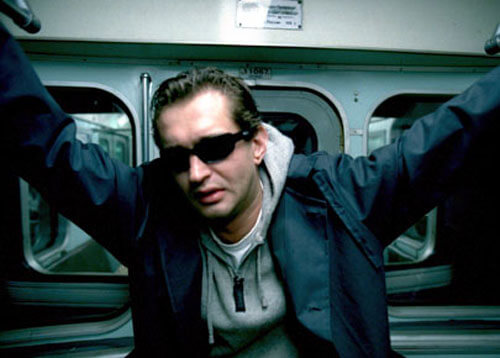
\includegraphics[width=\textwidth]{hub}
    \caption{Ты тоже их видишь? Смыслы...}
\end{figure}
% реклама
\begin{figure}[ht!]
    \centering
    
\includegraphics[width=\textwidth]{tea}
    \caption{Чай по-студенчески: без сахара и без заварки}
\end{figure}

\subsection{Recursive acronym}
\begin{flushleft}\parskip1em
    Рекурсивный акроним --- бэкроним (аббревиатура или акроним), который косвенно или напрямую ссылается на себя.\\
    Классика:\\
    ЛОМ --- лом обыкновенный металлический.\\
    GNU --- GNU's Not UNIX.

    \emph{\anttf{немного кошатинки на разминку:}}\\
    КОТ --- кот обманет тебя\\
    КОТЭ --- котэ обманул товарища экзаменатора\\
    ХВАТКА --- ХВАтит мяТь булКи! А!\\
    КРУТО --- круто разработал усовершенствование текущего опуса

    \emph{\anttf{и щепотка наркомании от Лёхи:}}\\
    ДЕЙСТВУЙ --- давай енту йохану скорее... также вувузелу у Йорика.\\
    ТИРЕ --- так и рождаются еноты.

    \emph{так и рождаются диалекты}\\
    STAR --- star to a rise\\
    \emph{если перевести rise как рассвет}
\end{flushleft}
% реклама
\begin{figure}[ht!]
    \centering
    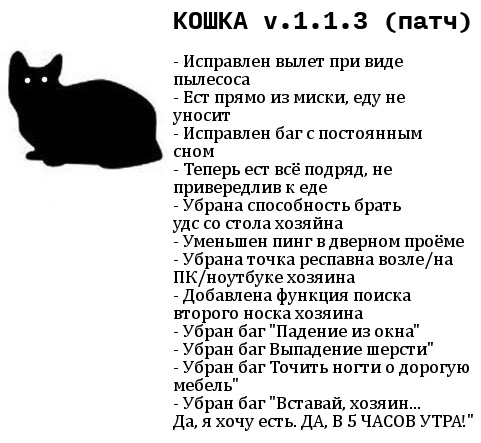
\includegraphics[width=\textwidth]{cat}
    \caption{Всего за \$ 1.99}
\end{figure}

\subsection{Порядочно разные предложения}
Идея: изменять смысл предложения изменяя порядок слов.\\

Сlassic (for example): I would not --- Would I not\\

Я не хочу этого --- Хочу не я этого --- Не этого хочу я --- Я хочу не этого --- Хочу этого я? Неееее...

\parskip2em

\framebox[0.9\textwidth][c]{
    Реклама дверей: \emph{обнаружься!}
}% висит над подземным переходом по ул. Мира около Комсы

\begin{epigraph}
    Я не сошёл с ума!\\
    \flushright{\normalfont Кипелов Валерий Александрович, 12 апреля 2001}
\end{epigraph}

\subsubsection{Поговорки на новый брак}

% тут потом надо красиво оформить диалог, с которого ноги начали расти, а ниже сами поговорки заоформить

не говори брак, пока не поломаешь
не всё коту качество, будет и брак
брак с возу — конвейеру легче
в ногах брака нет
глядит в книгу, видит брак
Без брака бракованные.
Брак в помощь.
Брак создал, брак и забрал.
Брак всё стерпит.
Была у собаки хата, брак пришел — она сгорела.
В ногах брака нет.
Там хорошо, где брака нет.
Вот где брак зарыт.
Вывести брак на чистую воду.
Где браки зимуют.
Брак - не тётка.
Два сапога - пара, а три - брак.
Дело пахнет браком.
Брак познаётся в беде.
Брака не хватает.
И швец, и жнец и бракоделец.

\framebox[0.9\textwidth][c]{
    А спонсор данной рубрики: \href{http://www.mista.ru/pogovorki.htm
}{Мои неуёмные}
}% надо спонсора переобозвать


